\documentclass{article}
\usepackage{graphicx}
\usepackage{amsmath}
\begin{document}
Robotic SLAM 
\section{Introduction}
Terms 

\begin{itemize}
    \item State estimation - find out the pose 
    \item Localisation - pose w.r.to landmark or map
    \item Mapping 
   \item navigation and motion planning - a star, wave front dijkstra 
\end{itemize}

\subsection{What is SLAM}
    Computing robot's poses and the map of the environment at the 
    same time.
\textbf{Localisation} : estimating robots location\\ 
\textbf{Mapping}      : building a MAP\\

\textbf{Given}

\begin{itemize}
    \item Robots control inputs   $$u_{1:T} = \{u_1,u_2,u_3....u_T\}$$
    \item Observations $$z_{1:T} = \{z_1,z_2,z_3,...,z_T\}$$
\end{itemize}

\textbf{Wanted}
\begin{itemize}
    \item Map of the environment $$m$$
    \item path of the Robot $$x_{0:T} = \{x_0,x_1,x_2,...,x_T\}$$
\end{itemize}

Using the robots control inputs we can predict the position of the robot.
From the observations $z_{1:T}$, we can calculate the position of the robot. 
Both the steps have some error associcated with it . Lets call the first
one the model noise and second one the sensor noise. So we have to associate 
a probability with both of them. The error accumulates over time(even if the
error in individual measurements is really small)\\

So in the probalistic terms our problem minimises to 
$$p(x_{0:T},m|z_{1:T},u_{1:T})$$


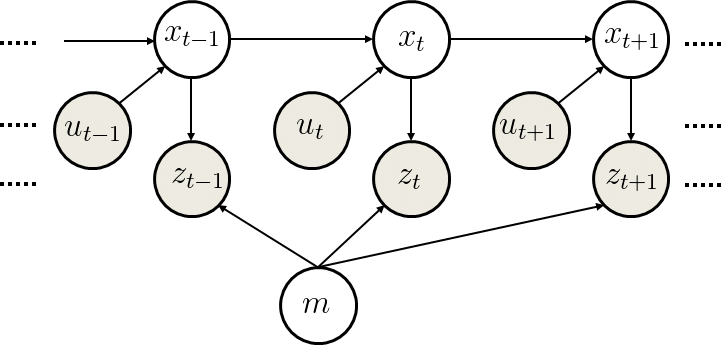
\includegraphics[width = \linewidth]{graphical_model.png}
\subsection{Full Slam vs online SLAM}
    \begin{itemize}
        \item Full SLAM estimates the entire path $$p(x_{0:T},m|z_{1:T},u_{1:T})$$
        \item Online SLAM estimates only the most recent pose $$p(x_{t},m|z_{1:T},u_{1:T})$$
    \end{itemize}
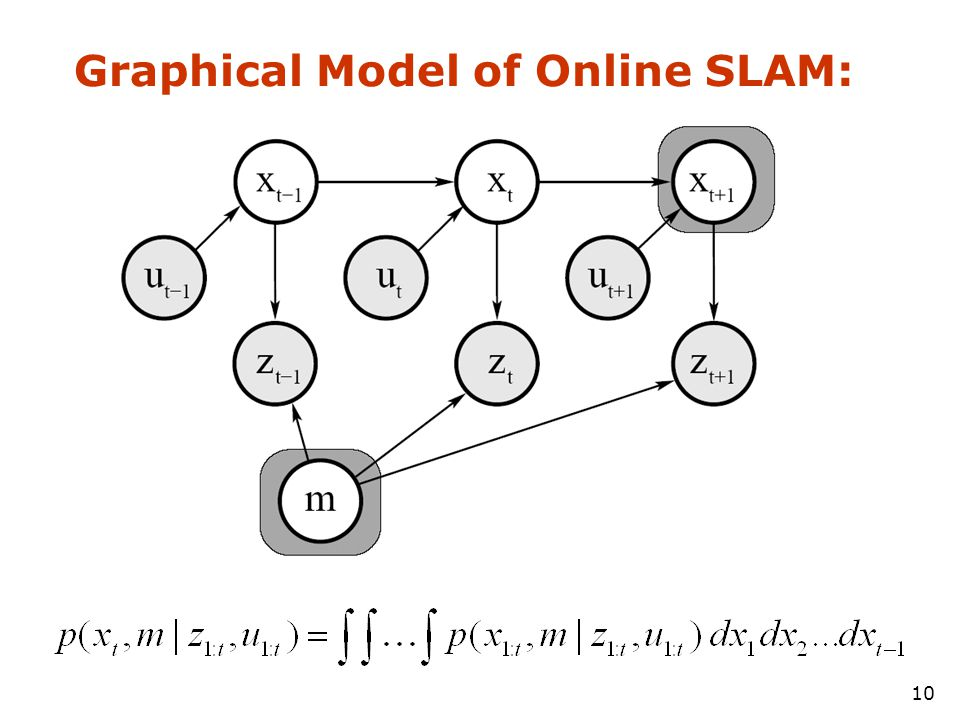
\includegraphics[width = \linewidth]{online_SLAM.jpg}

\subsection{Types of SLAM}
    occupancy maps created from lidars, sonars etc. - volumetric SLAM
    feature based approach - store features and localise based on that 
    volumetric SLAM maybe  better for navigation applications . 
    Topological representations vs geometric representations.
    Static vs dynamic features.
    Active - robot decides the path so as to build a map vs passive slam -
    may follow a fixed path i.e. path not optimised for mapping/ exploration
\section{Bayes Filter}
\subsection{State Estimation}
    \textbf{Goal} $p(x|z,u)$
    \newline
    \textbf{Recursive Bayes Filter} 

\begin{align*}  
    bel(x_t) & = p(x_t | z_{1:t},u_{1:t})\\
    & = \eta p(z_t|x_t,z_{1:t-1},u_{1:t}) * p(x_t | z_{1:t-1},u{1:t})\\
    & = \eta p(z_t|x_t) * p(x_t | z_{1:t-1},u{1:t})\\
    & = \eta p(z_t|x_t) \int_{x_{t-1}} p(x_t |x_{t-1}, z_{1:t-1},u_{1:t}) * p(x_{t-1}|z_{1:t-1}u_{1:t-1})dx_{t-1}\\
    & = \eta p(z_t|x_t) \int_{x_{t-1}} p(x_t |x_{t-1},u_t) * bel(x_{t-1})dx_{t-1}
 \end{align*}
 we can split this into predict and update steps where\\
 \textbf{Predict Step} 
 $$\overline{bel(x_t)} =  \int_{x_{t-1}} p(x_t |x_{t-1},u_t) * bel(x_{t-1})dx_{t-1}$$
 \textbf{Update Step} 
 $$bel(x_t) =  \eta * p(z_t | x_t) * \overline{bel(x_t)}$$


 \textbf{Bayes filter} gives a framework for recursive state estimation using
 the above equations. The actual realisation  may be kalman filtering , EKF or
 particle filter
 (Linear\ non linear motion models )
 (distributions)
 \textit{Kalman Filter} -  Gaussians , requires linear or linearised model 
 \textit{Particle filter} - Non-parametric , Arbitrary models
 
\end{document}
